% Created 2020-08-11 Tue 16:13
% Intended LaTeX compiler: pdflatex

\documentclass[a4paper,12pt]{article}
\usepackage[margin=2cm]{geometry}

\usepackage{hyperref}
\usepackage[utf8]{inputenc}
\usepackage{fixltx2e}
\usepackage{graphicx}
\usepackage{longtable}
\usepackage{float}
\usepackage{wrapfig}
\usepackage{rotating}
\usepackage[normalem]{ulem}
\usepackage{amsmath}
\usepackage{textcomp}
\usepackage{marvosym}
\usepackage{wasysym}
\usepackage{multicol}
\usepackage{amssymb}
\tolerance=1000
\usepackage{listings}
\usepackage[english]{babel}
\addto\captionsenglish{\renewcommand\contentsname{Outline}}
\hypersetup{linktoc = all, colorlinks = true, urlcolor = DodgerBlue4, citecolor = PaleGreen1, linkcolor = black}
\usepackage[UTF8, heading]{ctex}
\usepackage{xltxtra}
\usepackage{xeCJK}
\usepackage{lmodern}
\usepackage{verbatim}
\usepackage{float}
\usepackage{tikz}
\usepackage{wrapfig}
\usepackage{soul}
\usepackage{textcomp}
\usepackage{listing}
\usepackage{geometry}
\usepackage{algorithm}
\usepackage{algorithmic}
\usepackage{marvosym}
\usepackage{wasysym}
\usepackage{natbib}
\usepackage{fancyhdr}
\usepackage{fontspec,xunicode,xltxtra}
\usepackage{CJKnumb}
\usepackage{amsfonts}
\usepackage[default]{sourcecodepro}
\usepackage[T1]{fontenc}
\setCJKmainfont{SimSun} % 設置缺省中文字體
\setmainfont{Times New Roman} % 英文襯線字體
\setsansfont{Source Code Pro} % 英文無襯線字體
\setmonofont{Source Code Pro} % 英文等寬字體
\setCJKmainfont[Scale=0.9]{Adobe Heiti Std} % 中文字體
\setCJKmonofont[Scale=0.9]{Adobe Heiti Std}
\usepackage{color}
\RequirePackage{fancyvrb}
\usepackage{placeins}
\vspace{-0.2cm}
\usepackage{xcolor}
\hypersetup{pdfauthor={Name}}
\definecolor{dkgreen}{rgb}{0,0.6,0}
\definecolor{dred}{rgb}{0.545,0,0}
\definecolor{dblue}{rgb}{0,0,0.545}
\definecolor{lgrey}{rgb}{0.9,0.9,0.9}
\definecolor{gray}{rgb}{0.4,0.4,0.4}
\definecolor{darkblue}{rgb}{0.0,0.0,0.6}
\definecolor{bubbles}{rgb}{0.91, 1.0, 1.0}
\definecolor{foreground}{RGB}{220,220,204} % 淺灰
\definecolor{background}{RGB}{62,62,62} % 淺黑
\definecolor{preprocess}{RGB}{250,187,249} % 淺紫
\definecolor{var}{RGB}{239,224,174} % 淺肉色
\definecolor{string}{RGB}{154,150,230} % 淺紫色
\definecolor{type}{RGB}{225,225,116} % 淺黃
\definecolor{function}{RGB}{140,206,211} % 淺天藍
\definecolor{keyword}{RGB}{239,224,174} % 淺肉色
\definecolor{comment}{RGB}{180,98,4} % 深褐色
\definecolor{doc}{RGB}{175,215,175} % 淺鉛綠
\definecolor{comdil}{RGB}{111,128,111} % 深灰
\definecolor{constant}{RGB}{220,162,170} % 粉紅
\lstdefinelanguage{python}{
backgroundcolor=\color{bubbles},
basicstyle=\footnotesize \ttfamily \color{dblue} \small \mono \bfseries,
breakatwhitespace=false,
breaklines=true,
captionpos=b,
comment=[l]{\#},
morecomment=[s]{/*}{*/},
commentstyle=\color{comment} \slshape \small \itshape,
ndkeywords={boolean, throw, import, typeof, null, catch, switch, for, in, int, str, float, self, return, class, if ,elif, endif, while, do, else, True, False , catch, def},
ndkeywordstyle=\color{dred} \bfseries \small \mono,
identifierstyle=\color{black},
deletekeywords={...},
escapeinside={\%*}{*)},
frame=single,
frameround=tttt,
framesep=0pt,
rulecolor=\color{background},
morekeywords={BRIEFDescriptorConfig,string,TiXmlNode,DetectorDescriptorConfigContainer,istringstream,cerr,exit},
identifierstyle=\color{black},
stringstyle=\color{blue},
rulecolor=\color{black},
showspaces=false,
showstringspaces=false,
showtabs=false,
stepnumber=1,
tabsize=5,
title=\lstname,
}
\lstdefinelanguage{shell}{
backgroundcolor=\color{keyword},
basicstyle=\footnotesize \ttfamily \color{dblue} \small \mono \bfseries,
breakatwhitespace=false,
breaklines=true,
captionpos=b,
comment=[l]{\#},
morecomment=[s]{/*}{*/},
commentstyle=\color{comment} \slshape \small \itshape,
identifierstyle=\color{black},
deletekeywords={...},
escapeinside={\%*}{*)},
frame=single,
frameround=tttt,
framesep=0pt,
rulecolor=\color{background},
morekeywords={BRIEFDescriptorConfig,string,TiXmlNode,DetectorDescriptorConfigContainer,istringstream,cerr,exit},
identifierstyle=\color{black},
stringstyle=\color{blue},
rulecolor=\color{black},
showspaces=false,
showstringspaces=false,
showtabs=false,
stepnumber=1,
tabsize=5,
title=\lstname,
}
\usepackage{enumitem}
\setenumerate{noitemsep}
\setenumerate{nolistsep}
\setitemize{nolistsep}
\vspace{-\topsep}
\author{Yung Chin, Yen}
\date{\today}
\title{SwiftUI}
\begin{document}

\maketitle
\tableofcontents

\newpage

\section{iOS app 的開發界面: UIKit v.s. SwiftUI}
\label{sec:orgd284981}
\subsection{UIKit 與 SwiftUI 的差異性}
\label{sec:orga0c7f6b}
\begin{enumerate}
\item 系統需求
\label{sec:org66dae18}
UIKit 是從 Xcode1 就一直存在的 Framework;而 SwiftUI 則是 2019/6 WWDC 所發表的全新用來繪製 UI 的 Framework。因此,SwiftUI 必須搭配 iOS13+ 和 MacOS10.15+。\footnote{\href{https://medium.com/@mikru168/swiftui-\%E6\%B7\%BA\%E7\%8E\%A9-swiftui-\%E7\%94\%A8\%E5\%85\%B6\%E5\%BB\%BA\%E6\%A7\%8B\%E4\%B8\%80\%E7\%B0\%A1\%E5\%96\%AE\%E7\%9A\%84-app-2f2477bd49d7}{簡介 SwiftUI \& 用其建構一簡單的 APP }\\}\\
\item 底層語言
\label{sec:orga7610bb}
UIKit 底層仍為 Objecitve-C;而 SwiftUI 則是完完全全用 Swift 打造的 Framework。\\
\item 語法簡潔度
\label{sec:org215195e}
SwiftUI 產生一顯示文字的元件更精簡潔了。\\
\item 跨平台
\label{sec:org64bf009}
跨平台指的非跨 Android(但希望有那麼一天是可以支援的😀)。跨平台指的是使用 SwiftUI 所開發的專案,可以同時支援 macOS、watchOS、tvOS 等系統。引用一句 WWDC2019 SwiftUI 演講者所說的一句話。\\
\begin{quote}
Learn once, apply everywhere.\\
\end{quote}
\item Automatic Preview
\label{sec:orgad6c8bc}
這是此次 SwiftUI 最大的亮點之一,所謂 Automatic Preview,意思指的是即時預覽,即我們一邊調整程式碼的同時,也可以立即看到修改後的結果。\\
\item 自動支援進階功能
\label{sec:orgc451dfa}
SwiftUI 本身即支援 Dynamic Type、Dark Mode、 Localization 等等。這邊特別來講一下 UIKit 和 SwiftUI 在文字設定上有關於 Dark Mode 的差異,UIKit 若是無特別指定文字的顏色(意即使用 Default 的選項),在 Light Mode 字體會是白色;相對的在 Dark Mode 即會是白色,這點跟 SwiftUI 沒有特別的差異,但是 SwiftUI 除了 Default 外,還有 Secondary,如果還不喜歡的話,還有第三個選項,就是在 Assets 自行設定 Light Mode 和 Dark Mode 分別要顯示的顏色。\\
\begin{figure}[htbp]
\centering
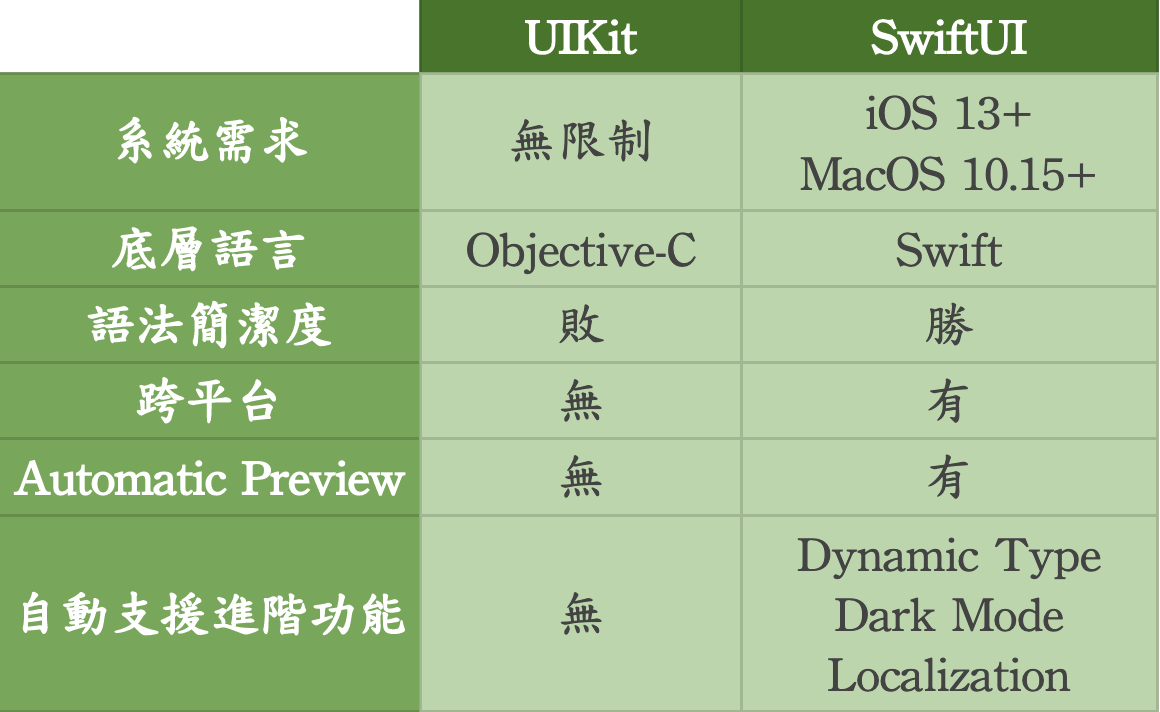
\includegraphics[width=300]{images/differences.png}
\caption{\label{fig:Diff-1}UIKit 與 SwiftUI 的差異性比較圖}
\end{figure}
\end{enumerate}

\subsection{SwiftUI vs UIKit: Benefits and Drawbacks}
\label{sec:org62673be}
\begin{enumerate}
\item Drawbacks of SwiftUI \footnote{\href{https://medium.com/@SteelKiwiDev/swiftui-vs-uikit-benefits-and-drawbacks-6a540cced684}{SwiftUI vs UIKit: Benefits and Drawbacks}\\\label{orge908e69}}
\label{sec:orgbc528df}
\begin{itemize}
\item It supports only iOS 13 and Xcode 11. By switching to them, you abandon users of older versions of iOS, which is a radical move devoid of concern for the user. But since Apple annually updates its list of supported iOS versions, I think SwiftUI will be used more over the next two years as users install the latest iOS version.\\
\item It’s still very young, so there isn’t much data on Stack Overflow. This means that you can’t get much help resolving complicated issues.\\
\item It doesn’t allow you to examine the view hierarchy in Xcode Previews.\\
\end{itemize}
\item Benefits of SwiftUI \textsuperscript{\ref{orge908e69}}
\label{sec:org9fe8909}
\begin{itemize}
\item It’s easy to learn, and the code is simple and clean.\\
\item It can be mixed with UIKit using UIHostingController.\\
\item It allows you to easily manage themes. Developers can easily add dark mode to their apps and set it as the default theme, and users can easily enable dark mode. Besides, it looks awesome.\\
\item SwiftUI provides mechanisms for reactive programming enthusiasts with BindableObject, ObjectBinding, and the whole Combine framework.\\
\item It offers Live Preview. This is a very convenient and progressive way to see the results of code execution in real time without having to build. I’m not sure if it somehow affects the processor. So far, I’ve noticed a delay provoked by the use of Live Preview, but I think Apple will soon make improvements.\\
\item SwiftUI no longer needs Interface Builder. It was replaced by Canvas, an interactive interface editor. When writing code, the visual part in Canvas is automatically generated, and when you create visual presentation elements, they automatically appear in the code.\\
\item Your application will no longer crash if you forget to update the @IBOutlet association with the variable.\\
\item There’s no AutoLayout or related problems. Instead, you use things like HStack, VStack, ZStack, Groups, Lists, and more. Unlike AutoLayout, SwiftUI always produces a valid layout. There’s no such thing as an ambiguous or unsatisfiable layout. SwiftUI replaces storyboards with code, making it easy to create a reusable view and avoid conflicts related with the simultaneous use of one project by the development team.\\
\end{itemize}
\end{enumerate}

\section{AppDelegate v.s. SceneDelegate}
\label{sec:org95913a5}
\begin{itemize}
\item SceneDelegate 為 Xcode11 所帶來的變化(可參考官方文件 WWDC2019),放在 SwiftUI 提似乎不太合適,但是在接下來在提到 SwiftUI App 的生命週期時會帶到,所以這邊就大概提一下。\\
\item AppDelegate 原來的職責為負責 App 的生命週期和 UI 生命週期,在 Xcode11 後,AppDelegate 將 UI 的生命週期(Scene Session)交給 SceneDelegate。原 Xcode10\\
\item 使用 Swift 為 User Interface 的專案 Launch 的生命週期為 AppDelegate → ViewController,而使用 SwiftUI 為 User Interface 的專案則變成為 AppDelegate → SceneDelegate → ContentView,原本應該出現在 AppDelegate 的 applicationWillEnterForeground(\_:) 等相關 App 到前、背景等相關的生命週期邏輯也都移至 SceneDelegate 裡了,method 名稱 application 的前綴字也都更改為 scene 了。\footnote{\href{https://www.appcoda.com.tw/swiftui-introduction/}{SwiftUI 初體驗: 建構一個簡單 App 讓你了解 SwiftUI 有多強大!}\\\label{orgd6a10cc}}\\
\end{itemize}

\subsection{SceneDelegate.swift}
\label{sec:orgbd74243}
\lstset{breaklines=true,language=swift,label= ,caption= ,captionpos=b,firstnumber=1,numbers=left}
\begin{lstlisting}
import UIKit
import SwiftUI

class SceneDelegate: UIResponder, UIWindowSceneDelegate {

    var window: UIWindow?

    func scene(_ scene: UIScene, willConnectTo session: UISceneSession, options connectionOptions: UIScene.ConnectionOptions) {
        // Use this method to optionally configure and attach the UIWindow `window` to the provided UIWindowScene `scene`.
        // If using a storyboard, the `window` property will automatically be initialized and attached to the scene.
        // This delegate does not imply the connecting scene or session are new (see `application:configurationForConnectingSceneSession` instead).

        // Create the SwiftUI view that provides the window contents.
        let contentView = ContentView()

        // Use a UIHostingController as window root view controller.
        if let windowScene = scene as? UIWindowScene {
            let window = UIWindow(windowScene: windowScene)
            window.rootViewController = UIHostingController(rootView: contentView)
            self.window = window
            window.makeKeyAndVisible()
        }
    }

    func sceneDidDisconnect(_ scene: UIScene) {
        // Called as the scene is being released by the system.
        // This occurs shortly after the scene enters the background, or when its session is discarded.
        // Release any resources associated with this scene that can be re-created the next time the scene connects.
        // The scene may re-connect later, as its session was not neccessarily discarded (see `application:didDiscardSceneSessions` instead).
    }

    func sceneDidBecomeActive(_ scene: UIScene) {
        // Called when the scene has moved from an inactive state to an active state.
        // Use this method to restart any tasks that were paused (or not yet started) when the scene was inactive.
    }

    func sceneWillResignActive(_ scene: UIScene) {
        // Called when the scene will move from an active state to an inactive state.
        // This may occur due to temporary interruptions (ex. an incoming phone call).
    }

    func sceneWillEnterForeground(_ scene: UIScene) {
        // Called as the scene transitions from the background to the foreground.
        // Use this method to undo the changes made on entering the background.
    }

    func sceneDidEnterBackground(_ scene: UIScene) {
        // Called as the scene transitions from the foreground to the background.
        // Use this method to save data, release shared resources, and store enough scene-specific state information
        // to restore the scene back to its current state.
    }
}

struct SceneDelegate_Previews: PreviewProvider {
    static var previews: some View {
        /*@START_MENU_TOKEN@*/Text("Hello, World!")/*@END_MENU_TOKEN@*/
    }
}
\end{lstlisting}

\begin{verbatim}
<stdin>:1:8: error: no such module 'UIKit'
import UIKit
       ^
\end{verbatim}

\section{UIKit}
\label{sec:org4ce8ea3}

\section{SwiftUI}
\label{sec:org01f2977}
\subsection{學習資源}
\label{sec:org2b9972e}
\begin{itemize}
\item \href{https://developer.apple.com/tutorials/swiftui/creating-and-combining-views}{SwiftUI Tutorials from Apple}\\
\end{itemize}

\subsection{使用 SwiftUI 開啟新專案 \textsuperscript{\ref{orgd6a10cc}}}
\label{sec:org68c3f29}
\begin{enumerate}
\item 首先,打開 Xcode,並點擊 Create new Xcode project。在 iOS 之下選擇 Single View App,並為專案命名。\\
\item 然後在下方勾選 Use SwiftUI 的選項,如果沒有勾選該選項的話,Xcode 會自動產生 storyboard 檔案(UIKit)。\\
\item Xcode 會自動幫你創建一個名為 ContentView.swif 的檔案,Xcode 會在程式碼的右邊呈現一個即時的預覽視窗(preview), 點選 resume 鈕生成預覽畫面(會花一點時間)。\\
\end{enumerate}

\begin{enumerate}
\item ContentView.swift
\label{sec:org161888f}
\lstset{breaklines=true,language=swift,label= ,caption= ,captionpos=b,firstnumber=1,numbers=left}
\begin{lstlisting}
import SwiftUI

struct ContentView: View {
    var body: some View {
        Text("文字")
    }
}

struct ContentView_Previews: PreviewProvider {
    static var previews: some View {
        ContentView()
    }
}
\end{lstlisting}
\end{enumerate}

\subsection{Text}
\label{sec:org9803c3c}
\begin{enumerate}
\item 改變 Text 的屬性
\label{sec:orgb96dcbb}
\begin{itemize}
\item 改變 component 有兩種方式:工具列、code\\
\item Attributes\\
\begin{itemize}
\item frame\\
\item foregroundColor\\
\item background\\
\item font\\
\end{itemize}
\end{itemize}

\begin{enumerate}
\item SwiftUI Inspector:
\label{sec:org937f96b}
\begin{enumerate}
\item on Text object (in preview screen): CMD + click\\
\item select \textbf{Show SwiftUI Inspector}\\
\item change \textbf{Text}, \textbf{Font}, \textbf{Color}\\
\item Monitor the corresponding code changes in code window\\
\end{enumerate}
\url{images/inspector-1.gif}\\
\item Inspector frame
\label{sec:org1c99f49}
\url{images/inspector-2.gif}\\
\item code
\label{sec:orgad8541d}
於 Text(``\ldots{}'')後加上屬性 function 或修改其他屬性\\
\url{images/inspector-3.gif}\\
\end{enumerate}
\end{enumerate}

\subsection{VStack}
\label{sec:org04d4e73}

一個以上的物件都要放在 Stack 中,Stack 與 Stack 可相互包含,加入方式有二:\\
\begin{enumerate}
\item 由工具列 drag: Xcode 會自動加入相對的 code
\label{sec:org6cf9367}
\url{images/vstack.gif}\\
\item coding
\label{sec:org6cb08be}
\lstset{breaklines=true,language=swift,label= ,caption= ,captionpos=b,firstnumber=1,numbers=left}
\begin{lstlisting}
import SwiftUI

struct ContentView: View {
    var body: some View {
        VStack {
            Text("第一行文字")
            Text("第二行文字")
        }
    }
}

struct ContentView_Previews: PreviewProvider {
    static var previews: some View {
        ContentView()
    }
}
\end{lstlisting}

\begin{figure}[htbp]
\centering

\includegraphics[width=300]{images/vstack-1.jpg}
\caption{\label{fig:VStack-1}VStack}
\end{figure}
\item SwiftUI 撰寫原則
\label{sec:org6e331c7}
\begin{itemize}
\item body 恆為只能 return 一物件。\\
\item 若有多個物件時,一定得放在 Stack 裡。\\
\end{itemize}
\end{enumerate}

\subsection{HStack}
\label{sec:orge0454bd}
\lstset{breaklines=true,language=swift,label= ,caption= ,captionpos=b,firstnumber=1,numbers=left}
\begin{lstlisting}
import SwiftUI

struct ContentView: View {
    var body: some View {
        HStack {
            VStack {
                Button("請按我") {
                    print("TEST")
                }
                .frame(width: 60, height: 30, alignment: .center)
                .foregroundColor(.white)
                .background(Color.green)
                Button("別亂按") {
                    print("QQ")
                }
            }
            VStack {
                Text("第一行文字")
                    .frame(width: 100, height: 30, alignment: .center   )
                    .foregroundColor(.white)
                    .background(Color.orange)
                Text("第二行文字")
                    .frame(width: 100, height: 30, alignment: .center)
                    .foregroundColor(.white)
                    .background(Color.red)
            }
        }
    }
}

struct ContentView_Previews: PreviewProvider {
    static var previews: some View {
        ContentView()
    }
}
\end{lstlisting}

\begin{figure}[htbp]
\centering

\includegraphics[width=300]{images/hstack-1.jpg}
\caption{\label{fig:HStack-1}HStack}
\end{figure}

\subsection{Image}
\label{sec:org65d563f}
影像來源可以是 System Image 或自行下載/編修的影像(Customized Image)\\
\begin{enumerate}
\item System Image
\label{sec:org7c567cf}
\begin{enumerate}
\item \href{https://developer.apple.com/design/human-interface-guidelines/sf-symbols/overview/}{SF Symbols }\footnote{\href{https://stackoverflow.com/questions/56514998/find-all-available-images-for-imagesystemname-in-swiftui}{Find all available images for Image(systemName:) in SwiftUI}\\}
\label{sec:orgfa6a63c}
\item 從 iOS 13 開始,Apple 介紹了一個名為 SFSymbols 的新功能。SF Symbols 這功能由 Apple 所設計,當中集合了 1500 多個可以在 App 之中使用的符號。\textsuperscript{\ref{orgd6a10cc}}
\label{sec:org840b993}
\item \href{https://developer.apple.com/design/resources/}{Download SF Symbols app}
\label{sec:org2da8446}
\item code
\label{sec:org84db0c0}
\lstset{breaklines=true,language=swift,label= ,caption= ,captionpos=b,firstnumber=1,numbers=left}
\begin{lstlisting}
import SwiftUI

struct ContentView: View {
    var body: some View {
        VStack {
            Text("System Image")
                .font(.headline)
                .foregroundColor(.orange)
            Image(systemName: "icloud")
            .resizable()
            .scaledToFit()
            .frame(width: 100, height: 80, alignment: .center)
        }
    }
}

struct ContentView_Previews: PreviewProvider {
    static var previews: some View {
        ContentView()
    }
}
\end{lstlisting}

\begin{verbatim}
<stdin>:9:13: error: 'init(systemName:)' is unavailable in macOS
            Image(systemName: "icloud")
            ^~~~~
SwiftUI.Image:7:12: note: 'init(systemName:)' has been explicitly marked unavailable here
    public init(systemName: String)
           ^
\end{verbatim}

\item Demo
\label{sec:orge826b5a}
\begin{figure}[htbp]
\centering

\includegraphics[width=300]{images/image-1.jpg}
\caption{\label{fig:Images-1}Images-1}
\end{figure}
\end{enumerate}

\item Customized Image 語法
\label{sec:org516819f}
\begin{enumerate}
\item Drag image into Project folder \textbf{Assets.xcassets}\\
\item Add following code\\
\end{enumerate}
\lstset{breaklines=true,language=swift,label= ,caption= ,captionpos=b,firstnumber=1,numbers=left}
\begin{lstlisting}
Image("ImageName") //file name in Assets.xcassets
  .resizable()
  .scaledToFit()
  .frame(width: 200, height: 160, alignment: .center)
\end{lstlisting}

\begin{verbatim}
<stdin>:1:1: error: use of unresolved identifier 'Image'
Image("ImageName") //file name in Assets.xcassets
^~~~~
\end{verbatim}

\item Image Attributes
\label{sec:orgc22f537}
\lstset{breaklines=true,language=swift,label= ,caption= ,captionpos=b,firstnumber=1,numbers=left}
\begin{lstlisting}
import SwiftUI

struct ContentView: View {
    var body: some View {
        VStack {
            Text("Albert Camus")
                .font(.title)
                .foregroundColor(.white)
                .background(Color.orange)
            Image("Albert-Camus")
                .resizable()
                .scaledToFill()
                .frame(width: 200, height: 200, alignment: .center)
                .clipShape(Circle())

        }
    }
}

struct ContentView_Previews: PreviewProvider {
    static var previews: some View {
        ContentView()
    }
}
\end{lstlisting}

\begin{figure}[htbp]
\centering
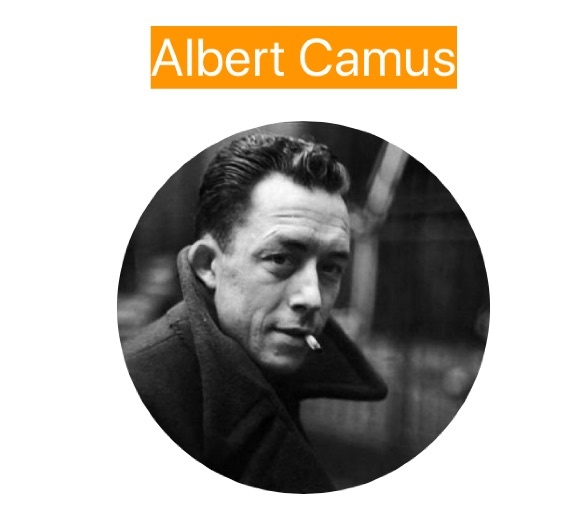
\includegraphics[width=300]{images/image-2.jpg}
\caption{\label{fig:Images-2}Images-2}
\end{figure}
\end{enumerate}

\subsection{Button}
\label{sec:org1a4f104}
\begin{enumerate}
\item 語法
\label{sec:org412ab74}
\lstset{breaklines=true,language=swift,label= ,caption= ,captionpos=b,firstnumber=1,numbers=left}
\begin{lstlisting}
//...
Button("Title") {
    //action
}

Button(action: <#T##() -> Void#>, label: <#T##() -> _#>)
//...
\end{lstlisting}

\begin{verbatim}
<stdin>:6:16: error: editor placeholder in source file
Button(action: <#T##() -> Void#>, label: <#T##() -> _#>)
               ^
<stdin>:6:42: error: editor placeholder in source file
Button(action: <#T##() -> Void#>, label: <#T##() -> _#>)
                                         ^
<stdin>:6:53: error: expected type for function result
Button(action: <#T##() -> Void#>, label: <#T##() -> _#>)
                                                    ^
<stdin>:2:1: error: use of unresolved identifier 'Button'
Button("Title") {
^~~~~~
<stdin>:6:1: error: use of unresolved identifier 'Button'
Button(action: <#T##() -> Void#>, label: <#T##() -> _#>)
^~~~~~
\end{verbatim}

\item 範例: 按下 Button,改變 Text title
\label{sec:orgaca7569}
\lstset{breaklines=true,language=swift,label= ,caption= ,captionpos=b,firstnumber=1,numbers=left}
\begin{lstlisting}
struct ContentView: View {
    @State private var title = "Hello SWiftUI"

    var body: some View {
        VStack {
            Text(verbatim: title)
                .padding(4)
                .foregroundColor(.white)
                .background(Color.gray)
            Button(action: {
                self.title = "Good Day"
            }) {
                Text("請按我1")
                    .foregroundColor(.white)
                    .padding(4)
                    .background(Color.blue)
            }
            Button("請按我2") {
                self.title = "Good night..."
            }
        }
    }
}
\end{lstlisting}

\begin{verbatim}
<stdin>:2:5: error: unknown attribute 'State'
    @State private var title = "Hello SWiftUI"
    ^
<stdin>:4:20: error: use of undeclared type 'View'
    var body: some View {
                   ^~~~
<stdin>:1:21: error: use of undeclared type 'View'
struct ContentView: View {
                    ^~~~
\end{verbatim}

\item Demo
\label{sec:orga9ee5fc}
\begin{figure}[htbp]
\centering

\includegraphics[width=300]{images/swbtn-1.jpg}
\caption{\label{fig:Button-1}Button}
\end{figure}
\end{enumerate}

\subsection{TextField}
\label{sec:org46d9d77}
\begin{enumerate}
\item 語法
\label{sec:orgf3c1d25}
\lstset{breaklines=true,language=swift,label= ,caption= ,captionpos=b,firstnumber=1,numbers=left}
\begin{lstlisting}
@State private var 變數="值"
TextField("提示文字", text: $變數)
\end{lstlisting}

\begin{verbatim}
<stdin>:2:33: error: '$' is not an identifier; use backticks to escape it
TextField("提示文字", text: $變數)
<stdin>:2:34: error: expected ',' separator
TextField("提示文字", text: $變數)
<stdin>:1:1: error: unknown attribute 'State'
@State private var 變數="值"
<stdin>:2:1: error: use of unresolved identifier 'TextField'
TextField("提示文字", text: $變數)
<stdin>:2:33: error: use of unresolved identifier '$'
TextField("提示文字", text: $變數)
\end{verbatim}

\item 範例: 於 TextField 輸入資料,顯示於 Text 中
\label{sec:org902f09a}
\lstset{breaklines=true,language=swift,label= ,caption= ,captionpos=b,firstnumber=1,numbers=left}
\begin{lstlisting}
import SwiftUI

struct ContentView: View {
    @State private var title = ""

    var body: some View {
        VStack {
            Text(verbatim: "Hello "+title)
            HStack {
                Text("Your Name: ")
                TextField("請輸入姓名:", text: $title)
            }
        }
    }
}

struct ContentView_Previews: PreviewProvider {
    static var previews: some View {
        ContentView()
    }
}
\end{lstlisting}

\item Demo
\label{sec:org644a968}
\begin{figure}[htbp]
\centering

\includegraphics[width=300]{images/txtfield-1.jpg}
\caption{\label{fig:Button-1}Button}
\end{figure}
\end{enumerate}

\section{Customize UI Components}
\label{sec:org800f38c}
SwiftUI 提供豐富的 modifier 幫助我們設計客製 UI 元件的樣式,諸如陰影,旋轉等效果皆可透過 modifier 實現,還可以搭配方便的拖曳加入相關程式碼。\footnote{\href{https://medium.com/\%E5\%BD\%BC\%E5\%BE\%97\%E6\%BD\%98\%E7\%9A\%84-swift-ios-app-\%E9\%96\%8B\%E7\%99\%BC\%E5\%95\%8F\%E9\%A1\%8C\%E8\%A7\%A3\%E7\%AD\%94\%E9\%9B\%86/\%E5\%AE\%A2\%E8\%A3\%BD-ui-\%E5\%85\%83\%E4\%BB\%B6\%E6\%A8\%A3\%E5\%BC\%8F\%E7\%9A\%84-swiftui-modifier-b31ff65c1f0d}{客製 UI 元件樣式的 SwiftUI modifier}\\}\\

\subsection{Text}
\label{sec:orge28b386}
\begin{enumerate}
\item Advanced Attributes \footnote{\href{https://medium.com/\%E5\%BD\%BC\%E5\%BE\%97\%E6\%BD\%98\%E7\%9A\%84-swift-ios-app-\%E9\%96\%8B\%E7\%99\%BC\%E5\%95\%8F\%E9\%A1\%8C\%E8\%A7\%A3\%E7\%AD\%94\%E9\%9B\%86/\%E5\%AE\%A2\%E8\%A3\%BD-ui-\%E5\%85\%83\%E4\%BB\%B6\%E6\%A8\%A3\%E5\%BC\%8F\%E7\%9A\%84-swiftui-modifier-b31ff65c1f0d}{客製 UI 元件樣式的 SwiftUI modifier}\\}
\label{sec:org4a50ae5}
\lstset{breaklines=true,language=swift,label= ,caption= ,captionpos=b,firstnumber=1,numbers=left}
\begin{lstlisting}
struct ContentView: View {
    var body: some View {
        Text("Example")
            .font(.title)
            .fontWeight(.bold)
            .foregroundColor(Color.white)
            .padding(4)
            .background(Color.gray)
            .cornerRadius(14.0)
            .rotationEffect(Angle(degrees: 15))
            .rotation3DEffect(Angle(degrees: 30), axis: (x: 10, y: 30, z: 30))
            .shadow(radius: 20)
    }
}
\end{lstlisting}

\begin{verbatim}
<stdin>:2:20: error: use of undeclared type 'View'
    var body: some View {
                   ^~~~
<stdin>:1:21: error: use of undeclared type 'View'
struct ContentView: View {
                    ^~~~
\end{verbatim}

\item Demo
\label{sec:orge491d73}
\begin{figure}[htbp]
\centering
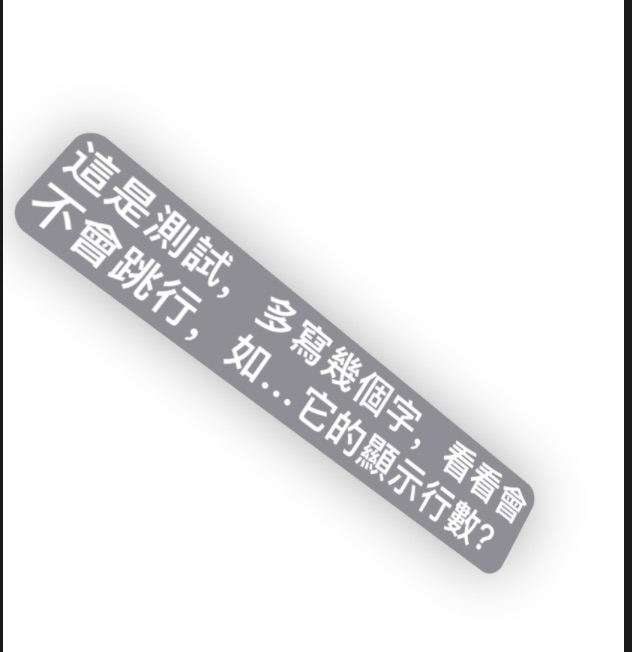
\includegraphics[width=300]{images/adv-text-attributes.jpg}
\caption{\label{fig:Adv-Text_Attributes}Text Attributes}
\end{figure}
\end{enumerate}

\subsection{Image}
\label{sec:orga1d9ac2}
\begin{enumerate}
\item Advanced Attributes \footnote{\href{https://medium.com/\%E5\%BD\%BC\%E5\%BE\%97\%E6\%BD\%98\%E7\%9A\%84-swift-ios-app-\%E9\%96\%8B\%E7\%99\%BC\%E5\%95\%8F\%E9\%A1\%8C\%E8\%A7\%A3\%E7\%AD\%94\%E9\%9B\%86/swiftui-\%E8\%A3\%81\%E5\%88\%87\%E5\%BD\%A2\%E7\%8B\%80\%E7\%9A\%84-clipshape-mask-4fc49b34141}{SwiftUI 裁切形狀的 clipShape \& mask}\\}
\label{sec:org0b81f33}
\lstset{breaklines=true,language=swift,label= ,caption= ,captionpos=b,firstnumber=1,numbers=left}
\begin{lstlisting}
import SwiftUI

struct ContentView: View {
    var body: some View {
        VStack {
            Text("Albert Camus")
                .font(.body)
                .foregroundColor(.white)
                .background(Color.orange)
            Image("Albert-Camus")
                .resizable()
                .scaledToFill()
                .frame(width: 100, height: 100, alignment: .center)
                .clipShape(Circle())
            Image(systemName: "alarm.fill")
                .resizable()
                .scaledToFill()
                .frame(width: 100, height: 100, alignment: .center)
            Image("Albert-Camus")
                .frame(width: 100, height: 100, alignment: .center)
                .mask(Image(systemName: "alarm.fill")
                    .resizable()
                    .scaledToFit())
                .shadow(radius: 20)
        }
    }
}

struct ContentView_Previews: PreviewProvider {
    static var previews: some View {
        ContentView()
    }
}

\end{lstlisting}

\begin{verbatim}
<stdin>:15:13: error: 'init(systemName:)' is unavailable in macOS
            Image(systemName: "alarm.fill")
            ^~~~~
SwiftUI.Image:7:12: note: 'init(systemName:)' has been explicitly marked unavailable here
    public init(systemName: String)
           ^
<stdin>:21:23: error: 'init(systemName:)' is unavailable in macOS
                .mask(Image(systemName: "alarm.fill")
                      ^~~~~
SwiftUI.Image:7:12: note: 'init(systemName:)' has been explicitly marked unavailable here
    public init(systemName: String)
           ^
\end{verbatim}

\item Demo
\label{sec:orgd2e4cf1}
\begin{figure}[htbp]
\centering
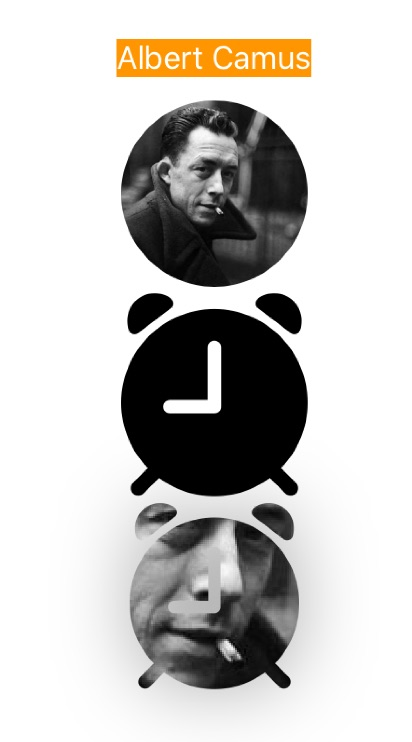
\includegraphics[width=300]{images/image-advanced-attributes.jpg}
\caption{\label{fig:Adv-Image-Attributes}Image Attributes}
\end{figure}
\end{enumerate}

\subsection{Button}
\label{sec:org972248d}
\begin{enumerate}
\item Advanced Attributes \footnote{\href{https://www.appcoda.com.tw/swiftui-border/}{SwiftUI 小技巧:利用 border 修飾符 輕鬆為按鈕或文本繪製邊框}\\}
\label{sec:org6cac3ea}
\lstset{breaklines=true,language=swift,label= ,caption= ,captionpos=b,firstnumber=1,numbers=left}
\begin{lstlisting}
import SwiftUI

struct ContentView: View {
    var body: some View {
        VStack(spacing: 5.0) {
            Text("Customized Button")
                .font(.body)
                .foregroundColor(.white)
                .background(Color.orange)
            Button(action: {
                print("Hello button tapped!")
            }) {
                Text("HI HI")
                    .fontWeight(.bold)
                    .font(.title)
                    .foregroundColor(.purple)
                    .padding()
                    .border(Color.purple, width: 5)
            }
            Button(action: {
                print("Hello button tapped!")
            }) {
                Text("Press me")
                    .fontWeight(.light)
                    .font(.title)
                    .foregroundColor(.green)
                    .padding(5)
                    .overlay(
                        Capsule(style: .continuous)
                            .stroke(Color.green, style: StrokeStyle(lineWidth: 3, dash: [10]))
                )
            }
        }
    }
}

\end{lstlisting}

\item Demo
\label{sec:org96017ad}
\begin{figure}[htbp]
\centering
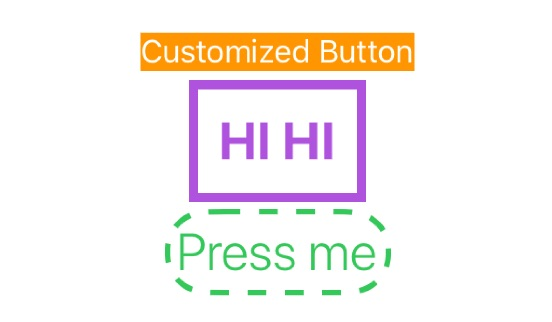
\includegraphics[width=300]{images/customized-button-1.jpg}
\caption{\label{fig:Adv-Button-Attributes}Button Attributes}
\end{figure}
\end{enumerate}

\section{Advanced Commponents}
\label{sec:org7f59c97}
\subsection{List}
\label{sec:org920e114}
\begin{enumerate}
\item 準備單一 cell 格式
\label{sec:org4a801c4}
\lstset{breaklines=true,language=swift,label= ,caption= ,captionpos=b,firstnumber=1,numbers=left}
\begin{lstlisting}
import SwiftUI

struct ContentView: View {
    var body: some View {
        HStack {
            Image(systemName: "book")
                .resizable()
                .frame(width: 30, height: 30, alignment: .center)
            VStack(alignment: .leading) {
                Text("Artificial Intelligence: A Modern Approach")
                    .multilineTextAlignment(.leading)
                    .foregroundColor(Color.green)
                Text("Stuart Russell and Peter Norvig")
                    .multilineTextAlignment(.leading)
                    .foregroundColor(Color.orange)
            }
        }
    }
}

\end{lstlisting}

\begin{verbatim}
<stdin>:6:13: error: 'init(systemName:)' is unavailable in macOS
            Image(systemName: "book")
            ^~~~~
SwiftUI.Image:7:12: note: 'init(systemName:)' has been explicitly marked unavailable here
    public init(systemName: String)
           ^
\end{verbatim}


\begin{figure}[htbp]
\centering

\includegraphics[width=300]{images/single-cell.jpg}
\caption{\label{fig:single-cell}Single cell}
\end{figure}
\item 轉入 List 格式
\label{sec:org7d5f204}
\begin{enumerate}
\item 將最外層的 VStack 加入 List 中
\label{sec:org80d5bdc}
\begin{figure}[htbp]
\centering
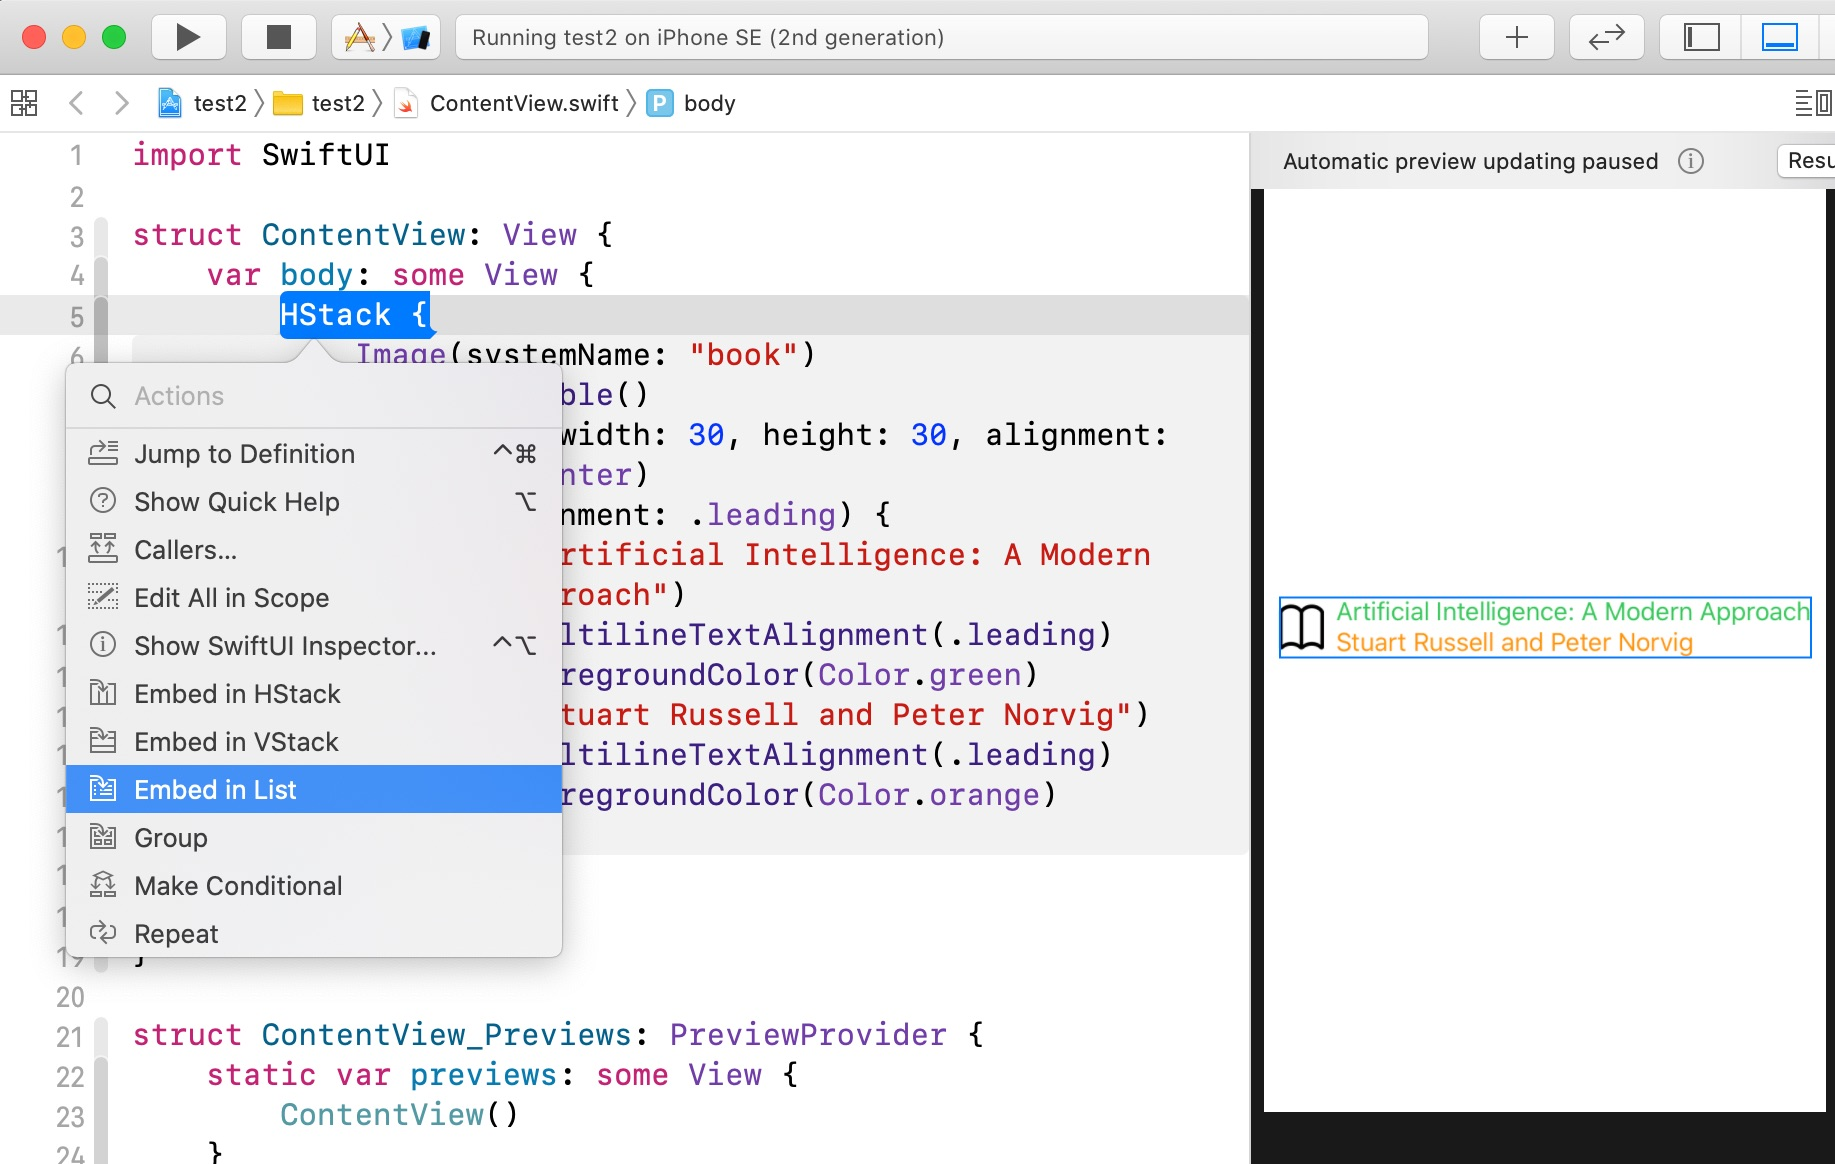
\includegraphics[width=400]{images/list-1.jpg}
\caption{\label{fig:list-1}List-1}
\end{figure}
\item list 語法
\label{sec:org84d10fa}
\lstset{breaklines=true,language=swift,label= ,caption= ,captionpos=b,firstnumber=1,numbers=left}
\begin{lstlisting}
import SwiftUI

struct ContentView: View {
    var body: some View {
        List(0 ..< 5) { item in
            Image(systemName: "book")
                .resizable()
                .frame(width: 30, height: 30, alignment: .center)
            VStack(alignment: .leading) {
                Text("Artificial Intelligence: A Modern Approach")
                    .multilineTextAlignment(.leading)
                    .foregroundColor(Color.green)
                Text("Stuart Russell and Peter Norvig")
                    .multilineTextAlignment(.leading)
                    .foregroundColor(Color.orange)
            }
        }
    }
}
\end{lstlisting}

\begin{verbatim}
<stdin>:6:13: error: 'init(systemName:)' is unavailable in macOS
            Image(systemName: "book")
            ^~~~~
SwiftUI.Image:7:12: note: 'init(systemName:)' has been explicitly marked unavailable here
    public init(systemName: String)
           ^
\end{verbatim}

\item 結果
\label{sec:org84e1d44}
\begin{figure}[htbp]
\centering
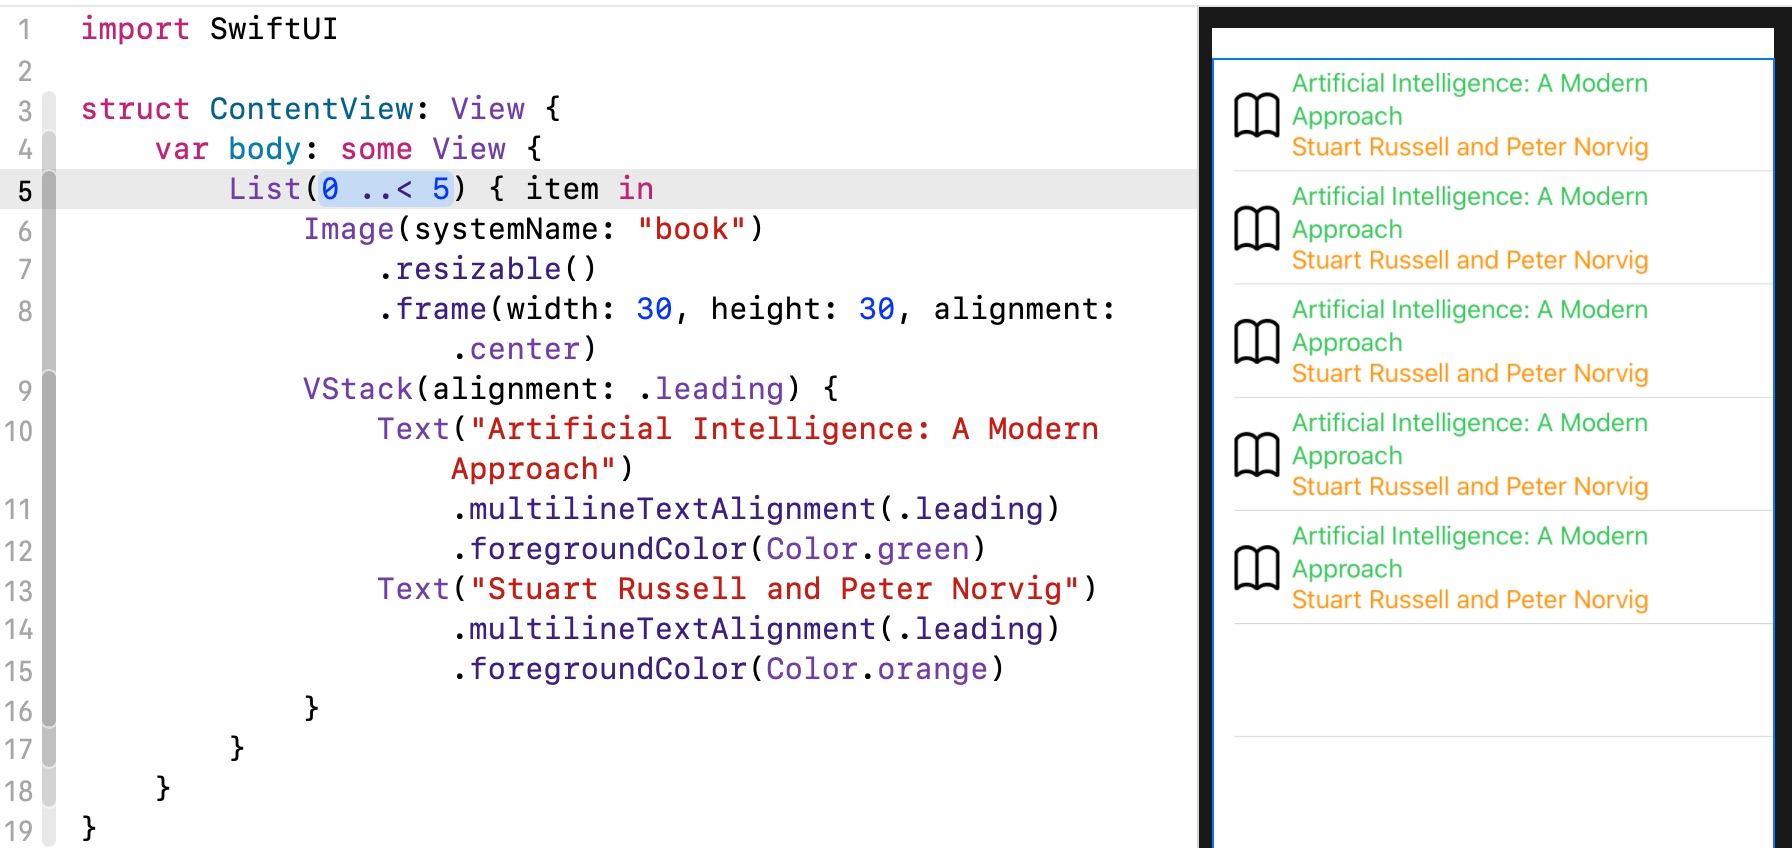
\includegraphics[width=400]{images/list-2.jpg}
\caption{\label{fig:list-2}List-2}
\end{figure}
\end{enumerate}
\item 建立 list 來源數據\textsuperscript{\ref{orgd6a10cc}}
\label{sec:org14ac36f}
\begin{verse}
In order to handle dynamic items, you must first tell SwiftUI how it can identify which item is which. This is done using the Identifiable protocol, which has only one requirement: some sort of id value that SwiftUI can use to see which item is which. \footnote{\href{https://www.hackingwithswift.com/quick-start/swiftui/how-to-create-a-list-of-dynamic-items}{How to create a list of dynamic items}\\}\\
\end{verse}
\lstset{breaklines=true,language=swift,label= ,caption= ,captionpos=b,firstnumber=1,numbers=left}
\begin{lstlisting}
import SwiftUI

//建立book struct
struct Book: Identifiable {
    var id = UUID()
    var title: String
    var author: String
    var image: String
}

struct ContentView: View {
    var books = [
      Book(id: UUID(), title: "地獄藍調", author: "李查德", image: "b1"),
      Book(id: UUID(), title: "至死方休", author: "李查德", image: "b2"),
      Book(id: UUID(), title: "一觸即發", author: "李查德", image: "b3"),
      Book(id: UUID(), title: "索命訪客", author: "李查德", image: "b4"),
      Book(id: UUID(), title: "闇夜回聲 ", author: "李查德", image: "b5")]

    //.....
}
\end{lstlisting}

\begin{verbatim}
<stdin>:11:8: error: type 'ContentView' does not conform to protocol 'View'
struct ContentView: View {
       ^
SwiftUI.View:5:20: note: protocol requires nested type 'Body'; do you want to add it?
    associatedtype Body : View
                   ^
\end{verbatim}

\item 將數據連結到列表中\textsuperscript{\ref{orgd6a10cc}}
\label{sec:org0639967}
\lstset{breaklines=true,language=swift,label= ,caption= ,captionpos=b,firstnumber=1,numbers=left}
\begin{lstlisting}
import SwiftUI

    //....
    var body: some View {
        List(books) { book in
            Image(book.image)
                .resizable()
                .frame(width: 40, height: 40, alignment: .center)
            VStack(alignment: .leading) {
                Text(book.title)
                    .multilineTextAlignment(.leading)
                    .foregroundColor(Color.green)
                Text(book.author)
                    .multilineTextAlignment(.leading)
                    .foregroundColor(Color.orange)
            }
        }
    }
}
\end{lstlisting}

\begin{verbatim}
<stdin>:19:1: error: extraneous '}' at top level
}
^
<stdin>:5:14: error: use of unresolved identifier 'books'
        List(books) { book in
             ^~~~~
\end{verbatim}

\item 結果
\label{sec:orgd0d4a2c}
\begin{figure}[htbp]
\centering
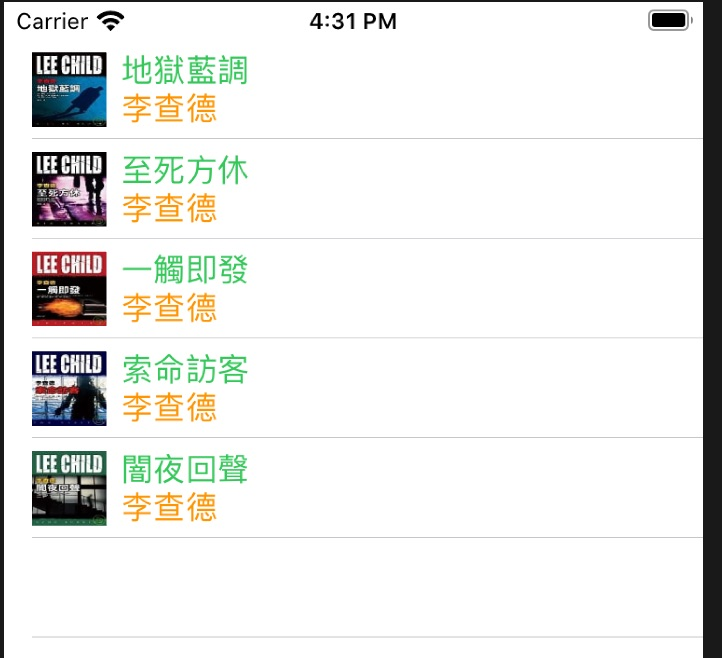
\includegraphics[width=300]{images/list-3.jpg}
\caption{\label{fig:list-3}List-3}
\end{figure}
\item 為什麼要加入 id 與 Identifiable
\label{sec:org7179784}
\begin{itemize}
\item Identifiable: 允許 Array 中有重複值\\
\item id: 明確區分重複值\\
\item UUID: 自動生成 unique 值\\
\item 詳細說明如\href{https://medium.com/flawless-app-stories/swiftui-dynamic-list-identifiable-73c56215f9ff}{SwiftUI - Dynamic List \& Identifiable}\\
\end{itemize}
\end{enumerate}

\subsection{Navigation bar}
\label{sec:org0ff3f7e}
\begin{itemize}
\item 於 body 中最外層的 component 之外加入 NavigationView\\
\item Title: navigationBarTitle()\\
\end{itemize}
\lstset{breaklines=true,language=swift,label= ,caption= ,captionpos=b,firstnumber=1,numbers=left}
\begin{lstlisting}
import SwiftUI
  ...

struct ContentView: View {
    ....
    var body: some View {
        NavigationView {
            List(books) { book in
                ...
                }
            }.navigationBarTitle(Text("書單"))
        }
    }
}
...
\end{lstlisting}

\begin{verbatim}
<stdin>:2:3: error: unary operator cannot be separated from its operand
  ...
  ^
     
<stdin>:4:1: error: expected expression
struct ContentView: View {
^
<stdin>:5:5: error: expected 'func' keyword in operator function declaration
    ....
    ^
    func 
<stdin>:5:9: error: expected '(' in argument list of function declaration
    ....
        ^
<stdin>:9:17: error: unary operator cannot be separated from its operand
                ...
                ^
                   
<stdin>:10:17: error: expected expression
                }
                ^
<stdin>:14:1: error: extraneous '}' at top level
}
^
<stdin>:15:1: error: expected expression after unary operator
...
^
<stdin>:15:4: error: expected expression
...
   ^
<stdin>:5:5: error: operator '....' declared in type 'ContentView' must be 'static'
    ....
    ^
    static 
<stdin>:5:5: error: operators must have one or two arguments
    ....
    ^
<stdin>:5:5: error: expected '{' in body of function declaration
    ....
    ^
<stdin>:5:5: error: member operator '....()' must have at least one argument of type 'ContentView'
    ....
    ^
<stdin>:8:18: error: use of unresolved identifier 'books'
            List(books) { book in
                 ^~~~~
\end{verbatim}

\begin{figure}[htbp]
\centering
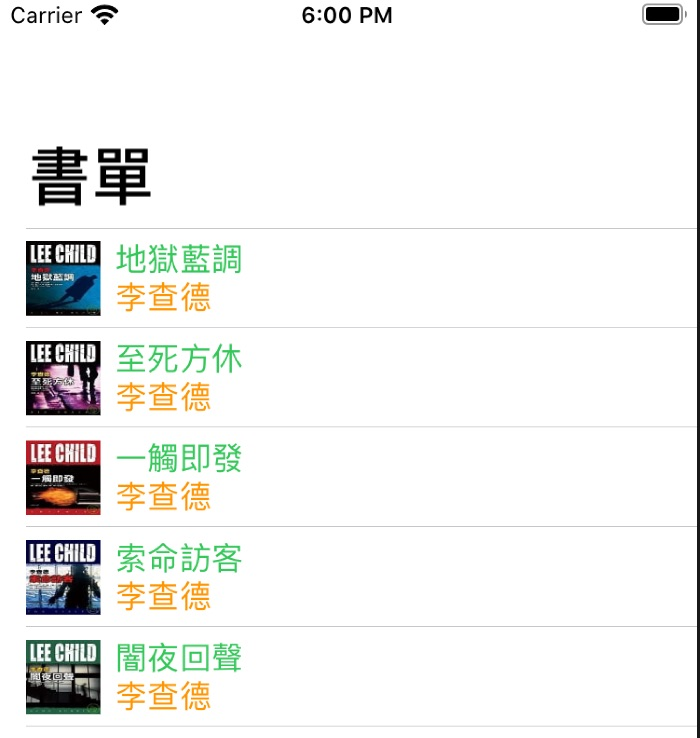
\includegraphics[width=300]{images/navigation-1.jpg}
\caption{\label{fig:Navigation-1}Navigation bar}
\end{figure}

\subsection{Button, Divider}
\label{sec:org300b4a8}
\lstset{breaklines=true,language=swift,label= ,caption= ,captionpos=b,firstnumber=1,numbers=left}
\begin{lstlisting}
//
//  ContentView.swift
//  uitest
//
//  Created by yen yung chin on 2020/7/29.
//  Copyright © 2020 Letranger.tw. All rights reserved.
//

import SwiftUI

struct ContentView: View {
    @State private var a = ""
    @State private var b = ""
    @State private var c = "Ans:"
    
    var body: some View {
        VStack {
            VStack {
                Divider()
                TextField("Number 1: ", text: $b)
                Divider()
                TextField("Number 2:", text: $a)
                Divider()
                Button("➕") {
                    let one = Int(self.a) ?? 0
                    let two = Int(self.b) ?? 0
                    self.c = "Ans: " + String(one + two)
                }
                .frame(width: 40, height: 30, alignment: .center)
                .foregroundColor(.white)
                .background(Color.green)
                .font(.largeTitle)
                Divider()
                Text(verbatim: c)
                    .foregroundColor(.gray)
            }
            .frame(width: 200, height: 160, alignment: .center)
            
        }
    }
}
\end{lstlisting}

\begin{figure}[htbp]
\centering
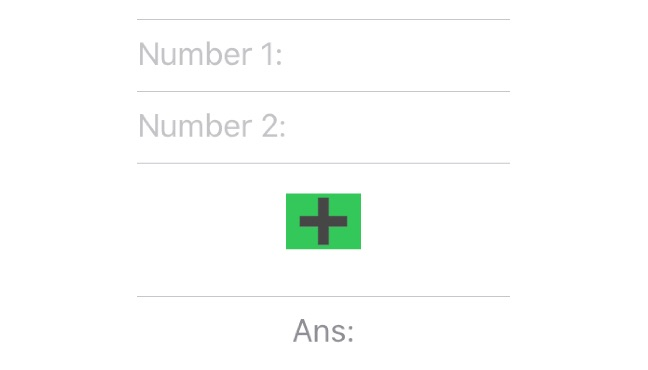
\includegraphics[width=300]{images/btn-1.jpg}
\caption{\label{fig:Button-1}Button}
\end{figure}

\subsection{background, opacity}
\label{sec:org1be7984}
\lstset{breaklines=true,language=swift,label= ,caption= ,captionpos=b,firstnumber=1,numbers=left}
\begin{lstlisting}
//
//  ContentView.swift
//  uitest
//
//  Created by yen yung chin on 2020/7/29.
//  Copyright © 2020 Letranger.tw. All rights reserved.
//

import SwiftUI

struct ContentView: View {
    @State private var a = ""
    @State private var b = ""
    @State private var c = "Ans:"

    var body: some View {
        VStack(alignment: .center) {
            Text("計算機")
            Divider()
            TextField("Number 1: ", text: $b)
            Divider()
            TextField("Number 2:", text: $a)
            Divider()
            Button("➕") {
                let one = Int(self.a) ?? 0
                let two = Int(self.b) ?? 0
                self.c = "Ans: " + String(one + two)
            }
            .frame(width: 40, height: 30, alignment: .center)
            .foregroundColor(.white)
            .background(Color.white)
            .font(.largeTitle)
            Divider()
            Text(verbatim: c)
                .foregroundColor(.black)


        }
        .padding(60)
        .background(Image("background").resizable().scaledToFill())
        .opacity(0.9)
    }
}
struct ContentView_Previews: PreviewProvider {
    static var previews: some View {
        ContentView()
    }
}


\end{lstlisting}

\begin{figure}[htbp]
\centering
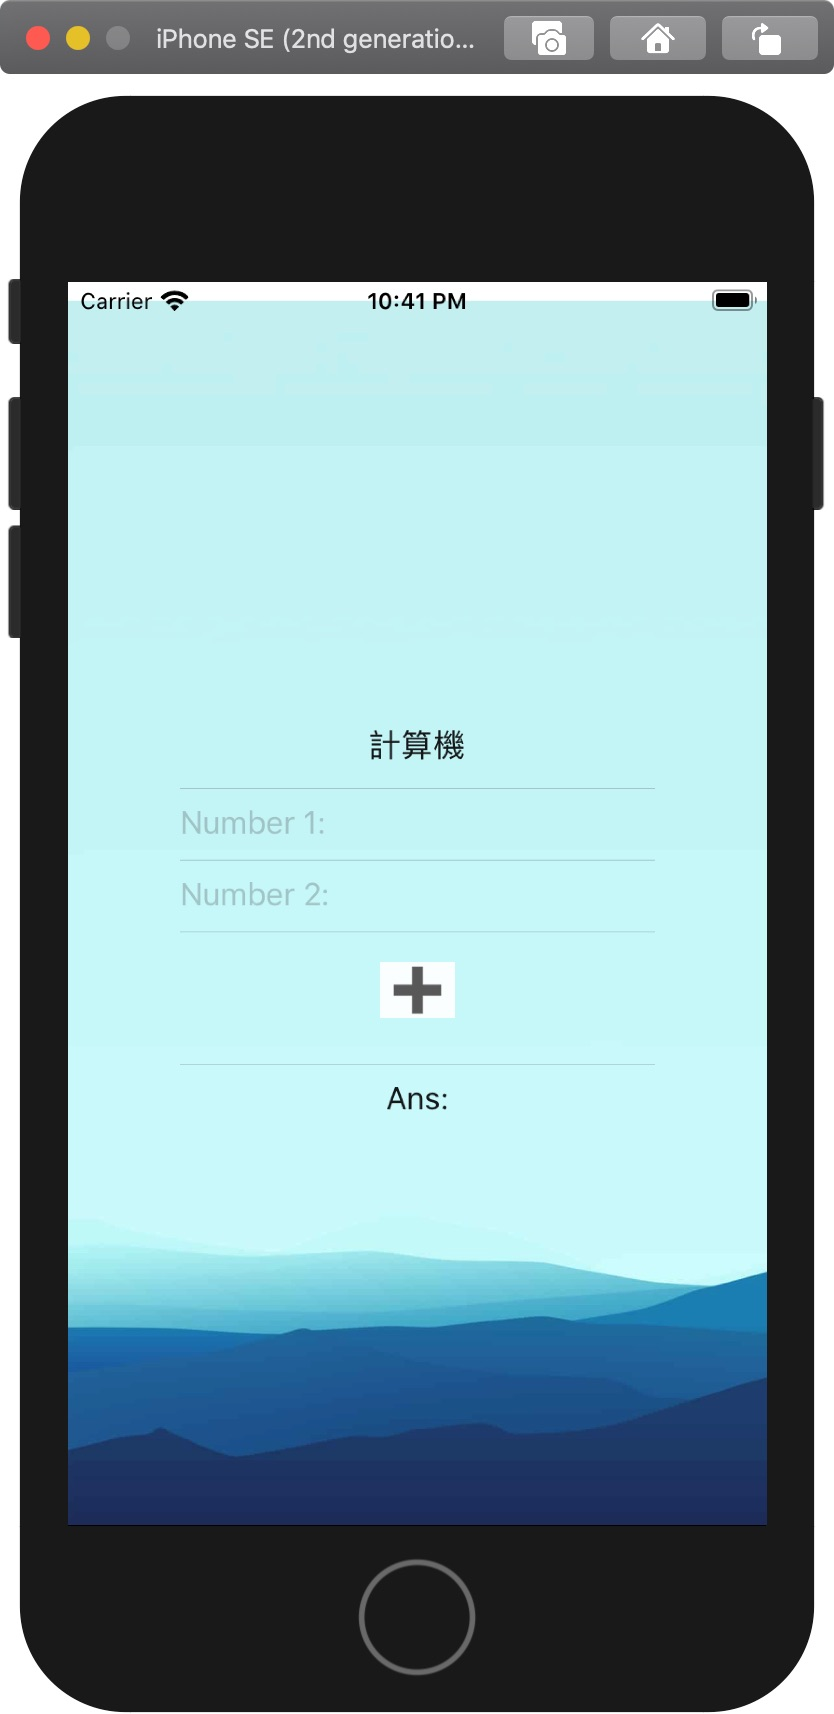
\includegraphics[width=300]{images/background-1.jpg}
\caption{\label{fig:Background-1}Background}
\end{figure}

\section{Struct, Class, and Enum}
\label{sec:orgd17c297}
\begin{verse}
struct, class, and enum are fundamentally important concepts for every iOS developer. It’s difficult to imagine common iOS apps without them. \footnote{\href{https://levelup.gitconnected.com/demystifying-struct-class-and-enum-in-swift-5-43dde089e96a}{Demystifying Struct, Class, and Enum in Swift 5}\\\label{orgbf6fe03}}\\
\end{verse}
\subsection{Structures}
\label{sec:org8b7cdbf}
\lstset{breaklines=true,language=swift,label= ,caption= ,captionpos=b,firstnumber=1,numbers=left}
\begin{lstlisting}
struct Birthday {
  var day: Int = 12
  var month: Int = 12
  var year: Double = 1999

  func myBirthday() {
  print("I've born in \(year).\(month).\(day)")
  }
}

struct Person {
  var firstName: String = "Abboskhon"
  var lastName: String = "Shukurullaev"
  var phoneNumber: String = 123456
  var emailAddress: String = "abbsh24@gmail.com"

  func myInfo() {
  print("My name is \(firstName) \(secondName). My phone number is \(phoneNumber) and email address is \(emailAddress)")
  }
}
\end{lstlisting}

\begin{verbatim}
<stdin>:14:29: error: cannot convert value of type 'Int' to specified type 'String'
  var phoneNumber: String = 123456
                            ^~~~~~
<stdin>:18:36: error: use of unresolved identifier 'secondName'
  print("My name is \(firstName) \(secondName). My phone number is \(phoneNumber) and email address is \(emailAddress)")
                                   ^~~~~~~~~~
\end{verbatim}

\begin{enumerate}
\item Mutating methods
\label{sec:orgefed3e7}
\begin{verse}
Structs have also got so-called mutating methods that play a role in updating the property values of a structure within an instance method. \textsuperscript{\ref{orgbf6fe03}}\\
\end{verse}
\lstset{breaklines=true,language=swift,label= ,caption= ,captionpos=b,firstnumber=1,numbers=left}
\begin{lstlisting}
struct Counter {
  var count: Int = 0

  mutating func increment() {
    count += 1
  }
  mutating func increment(by amount: Int) {
    count += amount
  }
  mutating func reset() {
    count = 0
  }
}
var counter = Counter()   //default is 0
counter.increment()       //becomes 1
counter.increment(by: 9)  //becomes 10
counter.reset()           //reset to 0
\end{lstlisting}
\end{enumerate}

\subsection{Classes}
\label{sec:orgfff6d50}
\begin{verse}
Classes and structures are very similar, and both can be used to define properties and methods. \textsuperscript{\ref{orgbf6fe03}}\\
\end{verse}
\begin{enumerate}
\item Inheritance \& Override methods and properties
\label{sec:orgb60a314}
\begin{verse}
The biggest difference that structs do not have is hierarchical relations. Classes can have parent classes, that are called superclass, and child classes, that are called subclasses. \textsuperscript{\ref{orgbf6fe03}}\\
\end{verse}
\lstset{breaklines=true,language=swift,label= ,caption= ,captionpos=b,firstnumber=1,numbers=left}
\begin{lstlisting}
class Animals {
    func animals() {
        print("Animals are mainly of 3 types: Land Animals, Sea animals, Air Animals")
    }
}

class LandAnimals: Animals {
    override func animals() {
        print("Land animals are cats, sheeps, horses.")
    }
}

class Cat: LandAnimals {
    override func animals() {
        print("I am a cat and I am a land animal.")
    }
}
\end{lstlisting}
\end{enumerate}

\subsection{結構跟類的比較 (Comparing Structures and Classes) \footnote{\href{https://ithelp.ithome.com.tw/articles/10220520}{ Day 10: [Swift] 結構和類 (Struct and Class) }\\\label{org3a9738d}}}
\label{sec:org7ddd4a7}
\begin{enumerate}
\item 在 Swift 中的結構與類有許多相同之處,兩者皆能:
\label{sec:orgcb30043}
\begin{itemize}
\item 定義屬性來儲存值\\
\item 定義方法來提供功能\\
\item 定義下標來提供訪問他們用下標語法的值\\
\item 定義初始化器來設定他們的初始狀態\\
\item 可被擴展以擴展其功能,超越預設的實現\\
\item 符合協議以提供某種標準功能\\
\end{itemize}
\item 類具有的附加功能,但結構沒有:
\label{sec:org65cc083}
\begin{itemize}
\item 繼承使一個類能夠繼承另一個的特性\\
\item 類型轉換使我們可以在運行時檢查和解釋類實例的類型\\
\item 反初始化器允許類的實例釋放它已分配的任何資源\\
\item 引用計數允許對類實例的多個引用\\
\end{itemize}
\item 結構和列舉是值型別 (Structures and Enumerations Are Value Types)
\label{sec:org5f98dca}
值型別是一種其值在被賦值給變數或常數時被複製,或者在傳遞給函數時被複製。實際上,Swift 的整數、浮點數、布林值、字符串、數組和字典中的所有基本型別都是值型別,並且在幕後實現為結構。所有結構和列舉都是 Swift 中的值型別。這代表著我們創建的任何結構和列舉實例以及它們作為屬性的任何值類型在代碼中傳遞時始終會被複製。\textsuperscript{\ref{org3a9738d}}\\
\begin{enumerate}
\item 範例
\label{sec:org574b3e1}
\lstset{breaklines=true,language=swift,label= ,caption= ,captionpos=b,firstnumber=1,numbers=left}
\begin{lstlisting}
struct Resolution {
    var width = 0
    var height = 0
}

let hd = Resolution(width: 1920, height: 1080)
var cinema = hd

cinema.width = 2048

print("cinema is now \(cinema.width) pixels wide")
// Prints "cinema is now 2048 pixels wide"

print("hd is still \(hd.width) pixels wide")
// Prints "hd is still 1920 pixels wide"
\end{lstlisting}

\begin{verbatim}
cinema is now 2048 pixels wide
hd is still 1920 pixels wide
\end{verbatim}


由上述例子可知,當 cinema 被賦予 hd 當前的值,儲存在 hd 的值被複製到新 cinema 的實例。最後結果兩個擁有相同值但完全不同的實例,所以當修改 cinema.width = 2048 的時候,並不會影響儲存在 hd 中的 width。\textsuperscript{\ref{org3a9738d}}\\
\begin{figure}[htbp]
\centering
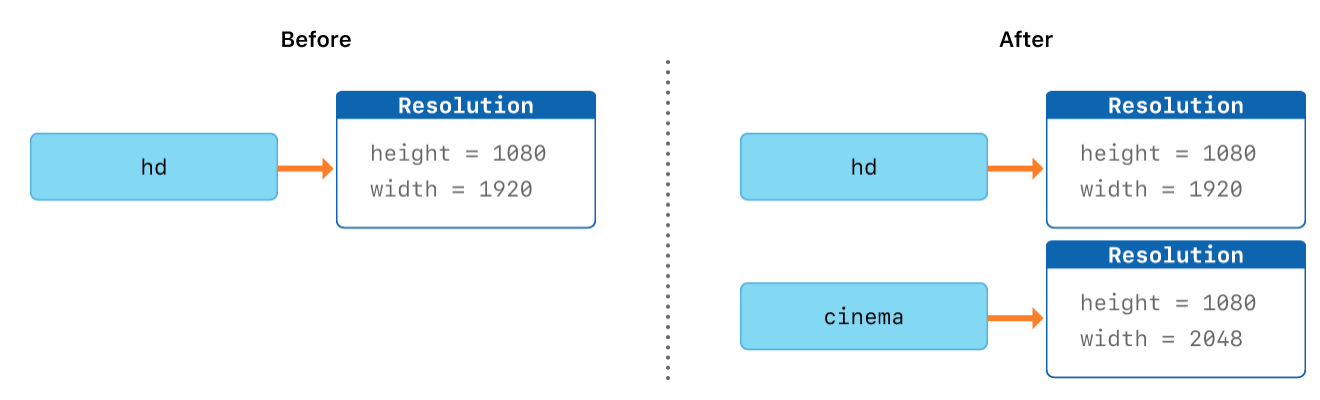
\includegraphics[width=400]{images/struct.png}
\caption{\label{fig:Structure}Struct value type}
\end{figure}
\end{enumerate}
\item 類是參考型別 (Classes Are Reference Types)
\label{sec:org460979b}
不同於值型別,當參考型別被指定給一個變數或常數,或是傳遞進一個函數的時候,並不會被複製。參考型別非副本,是使用相同存在的實例。\textsuperscript{\ref{org3a9738d}}\\
\begin{enumerate}
\item 範例
\label{sec:org90a49b0}
\lstset{breaklines=true,language=swift,label= ,caption= ,captionpos=b,firstnumber=1,numbers=left}
\begin{lstlisting}
class VideoMode {
    var interlaced = false
    var frameRate = 0.0
    var name: String?
}

let tenEighty = VideoMode()

tenEighty.interlaced = true
tenEighty.name = "1080i"
tenEighty.frameRate = 25.0

let alsoTenEighty = tenEighty
alsoTenEighty.frameRate = 30.0

print("The frameRate property of tenEighty is now \(tenEighty.frameRate)")
// Prints "The frameRate property of tenEighty is now 30.0"
\end{lstlisting}

\begin{verbatim}
The frameRate property of tenEighty is now 30.0
\end{verbatim}


由上述例子可知,當 alsoTenEighty 被指定為 tenEighty,並且修改 alsoTenEighty.frameRate = 30.0 時,也會更動到 tenEighty.frameRate 的值。\textsuperscript{\ref{org3a9738d}}\\
\begin{figure}[htbp]
\centering
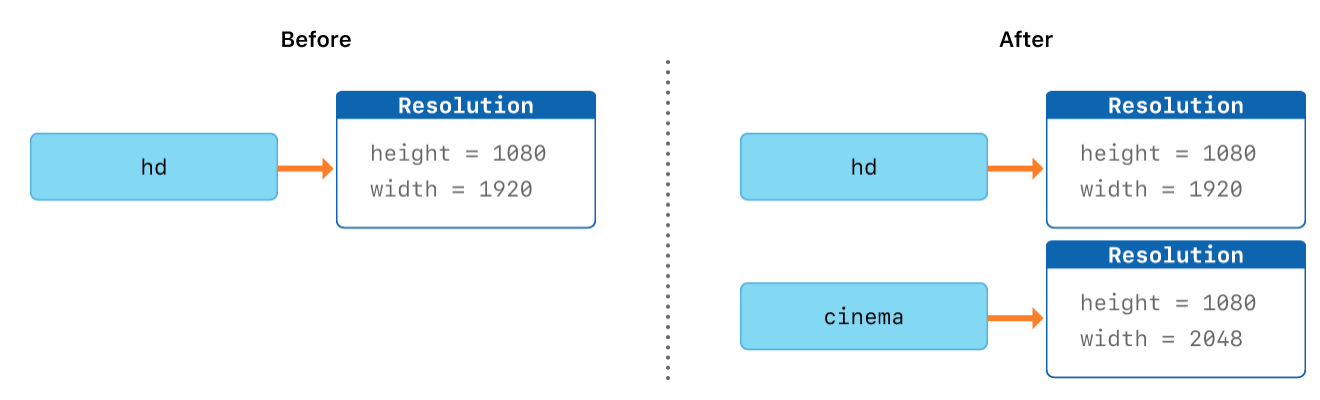
\includegraphics[width=400]{images/class.png}
\caption{\label{fig:Class-1}Class Reference type}
\end{figure}
\end{enumerate}
\end{enumerate}

\subsection{Enumerations}
\label{sec:orgaa61e8f}
\begin{verse}
Enumerations are different from structs and classes. Enum is a special Swift type that defines a common type for a group of related values. Then, enums can be interacted with other data types such as a switch, if statements, and others. \textsuperscript{\ref{orgbf6fe03}}\\
\end{verse}
從 Swift 3 開始,我們的 enum 內設定的情境字串要以小寫字母開頭。\\
\lstset{breaklines=true,language=swift,label= ,caption= ,captionpos=b,firstnumber=1,numbers=left}
\begin{lstlisting}
//1 representation of enum
enum DownloadStatus {
    case downloading
    case finished
    case failed
    case cancelled
}

var currentStatus = DownloadStatus.downloading

switch currentStatus {
case .downloading:
    print("Downloading...")

case .finished:
    print("Just finished the download...")

case .failed:
    print("Failed to download the file...")

case .cancelled:
    print("The download is cancelled...")
}
\end{lstlisting}

\begin{verbatim}
Downloading...
\end{verbatim}


\begin{verse}
此時,你可能會想,為什麼需要使用 enum 來定義多個情況,而不選擇宣告一個包含四個情境項目的 array,如下圖所示:\\
\vspace*{1em}
let downloadStatus = [“downloading”, “finished”, “failed”, “cancelled”]\\
let currentStatus = downloadStatus[0]\\
\vspace*{1em}
你可以這樣做沒錯,但是如此一來會有兩個缺點,首先,你可能會不知道 downloadStatus[0]代表什麼,除非你引用 downloadStatus array,若是比較 downloadStatus[0]與 DownloadStatus.downloading 這兩種表達方式,很明顯的是後者的可讀性比較高。\\
\vspace*{1em}
其次,因為 currentStatus 是 String 類型,變量可以被賦予任何字符串值,無法將它限制為 “downloading”, “finished”, “failed” 以及 “cancelled”,除非執行一些額外的驗證。反之,如果使用 enum,我們可以將 myDirection 限制在 .downloading、.finished、.failed 或 .cancelled 等四種情境之一,不會出現其他意料之外的情況。 \footnote{\href{https://appcoda.com.tw/mastering-swift/}{精通Swift:列舉、閉包、泛型、Protocols和高階函數}\\}\\
\end{verse}

\subsection{結構和類之間的選擇 (Choosing Between Structures and Classes)}
\label{sec:org294a42e}
\begin{verse}
總的來說,用 class 來定義資料物件的話,就好像是在用雲端共享文件一樣:每個人的螢幕上都會有一份文件可以編輯,但這個文件並沒有存在電腦裡,而是跟雲端的版本連線,所以所有的變動都是直接在雲端版本上更新的。好處是方便,壞處是誰修改了甚麼東西經理不會知道(class 本身沒有帳號功能!)。\\
\vspace*{1em}
用 struct 的話,則是像傳統的離線文件檔案一樣。一開始文件只有經理有,而如果他想要讓手下小美去修改文件的話,他就需要拷貝一份檔案給小美。小美修改完檔案後,必須把它交還給經理,然後經理再決定要不要用修改過的檔案取代原本的文件。\footnote{\href{https://www.appcoda.com.tw/swift-class/}{Swift Class vs Struct:設計 Model 時,該用 Struct 還是 Class 呢?}\\\label{org5073ec5}}\\
\end{verse}
\begin{figure}[htbp]
\centering
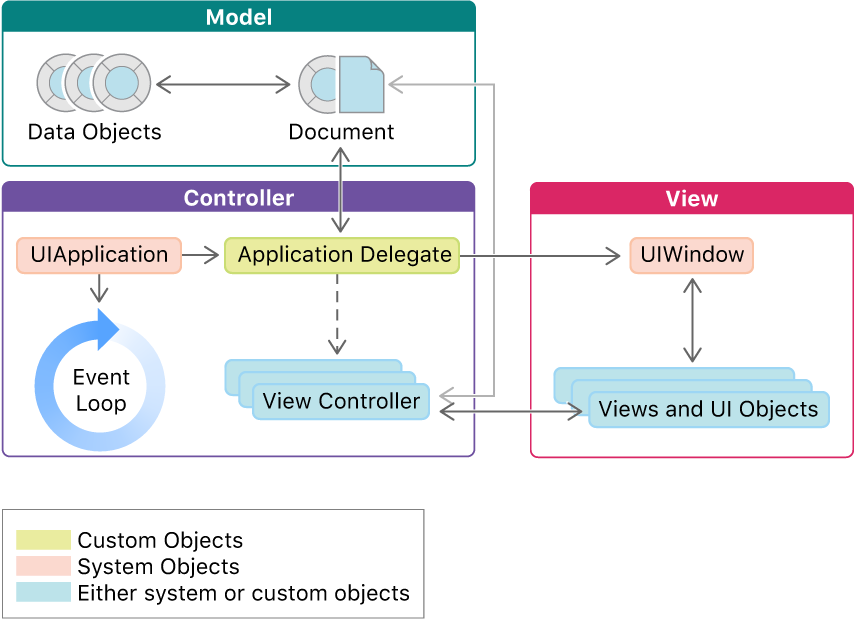
\includegraphics[width=400]{images/mvc-1.png}
\caption{\label{fig:MVC}MVC}
\end{figure}
\begin{itemize}
\item 在 MVC 架構中,Model 包含了 Data Objects 與 Document,其中 Documents 包含所有的資料管理者元件(如 Core Data 的 NSManagedObjectContext,或是任何負責下載、上傳資料物件的網路層元件,如自訂的 NetworkManager)。\\
\item Document 最好是用 class 來定義,因為它肩負了許多溝通的工作。Data Objects 則是資料的代表,要用 class 或 struct 來定義都可以。\\
\item 用 class 定義 Data Objects 的話,任何變動只要執行一次就可以了,因為它的實體只會有一個。然而,用 struct 定義的話,則需要將變動手動套用到文件所管理的那份實體,好讓整個 app 都能使用最新的資料。這雖然寫起來較為囉唆,卻讓閱讀與維護更為簡單(可以確定是在哪裡被變更資料)。\textsuperscript{\ref{org5073ec5}}\\
\end{itemize}
\begin{enumerate}
\item 選擇原則
\label{sec:org1efa312}
\begin{itemize}
\item Choose Structures by Default\\
\item Use Classes When You Need Objective-C Interoperability\\
\item Use Classes When You Need to Control Identity\\
\item Use Structures When You Don't Control Identity\\
\end{itemize}
\end{enumerate}

\section{Protocols}
\label{sec:org404fe19}
對任何程式開發來說,減少重覆的 code,把權責明確分開,讓 code 維護性變好,是非常重要的課題。而在現今的軟體開發模式中,有許多方法可以做到這點,最為人所知的一個模式,就是利用繼承 (Inheritance),把會重覆利用的部份放在母類別,讓其它子類別去繼承。另外一種做法,則是利用 Composition Pattern,將功能做成組件分出來,讓需要的模組去組合取用。\footnote{\href{https://www.appcoda.com.tw/protocol-extension/}{利用 Protocol Extension 減少重覆的 Code 大大增強 Code 的維護性}\\}\\
\begin{verse}
A protocol defines a blueprint of methods, properties, and other requirements that suit a particular task or piece of functionality. The protocol can then be adopted by a class, structure, or enumeration to provide an actual implementation of those requirements. Any type that satisfies the requirements of a protocol is said to conform to that protocol. \footnote{\href{https://docs.swift.org/swift-book/LanguageGuide/Protocols.html}{Protocols}\\}\\
\end{verse}

協定提供類型可以做的資訊,Classes 和 structs 則提供物件的資訊,協定則提供物件將會執行的動作。\footnote{\href{https://www.appcoda.com.tw/swift-protocol/}{Swift開發指南:Protocols與Protocol Extensions的使用心法}\\}\\
\begin{verse}
協定是 Swift 一個重要的特性,它會定義出為了完成某項任務或功能所需的方法、屬性,但是本身不會實作這些任務跟功能,而僅僅只是表達出該任務或功能的名稱。協定為方法、屬性、以及其他特定的任務需求或功能定義藍圖。協定可被 class、struct、或 enum 類型採納以提供所需功能的具體實現。滿足了協定中需求的任意類型都叫做遵循了該協定。\\
\vspace*{1em}
除了指定遵循類型必須實現的要求外,你可以擴展一個協定以實現其中的一些需求或實現一個符合類型的可以利用的附加功能。\footnote{\href{https://ithelp.ithome.com.tw/articles/10197366}{Day-29 Swift 語法(25) - 協定 Protocol}\\}\\
\end{verse}

\subsection{範例}
\label{sec:org4e67f78}
\begin{enumerate}
\item 版本 1
\label{sec:orgebc97bc}
本例中有兩個 struct: Song, Album 以及一個 class 用來播放 Song 或 Album,原本的 Player 要為不同的 struct 寫不同的 func,而且程式碼大多重複。\\
\lstset{breaklines=true,language=swift,label= ,caption= ,captionpos=b,firstnumber=1,numbers=left}
\begin{lstlisting}
import Cocoa
import AVKit

struct Song {
    var name: String
    var album: Album
    var audioURL: URL
    var isLiked: Bool
}

struct Album {
    var name: String
    var imageURL: URL
    var audioURL: URL
    var isLiked: Bool
}

class Player {
    private let avPlayer = AVPlayer()

    func play(_ song: Song) {
        let item = AVPlayerItem(url: song.audioURL)
        avPlayer.replaceCurrentItem(with: item)
        avPlayer.play()
    }

    func play(_ album: Album) {
        let item = AVPlayerItem(url: album.audioURL)
        avPlayer.replaceCurrentItem(with: item)
        avPlayer.play()
    }
}
\end{lstlisting}

\item 版本 2
\label{sec:orga6c1aaa}
宣告一個 protocol,定義 audioURL 變數(read only),然後令兩個 struct 皆遵循該 protocol(方式有二),如此,原本的 Player class 中的 play func 就能只寫一次。\\
\lstset{breaklines=true,language=swift,label= ,caption= ,captionpos=b,firstnumber=1,numbers=left}
\begin{lstlisting}
import Cocoa
import AVKit

protocol Playable {
    var audioURL: URL { get }
}

struct Song: Playable {
    var name: String
    var album: Album
    var audioURL: URL
    var isLiked: Bool
}

struct Album {
    var name: String
    var imageURL: URL
    var audioURL: URL
    var isLiked: Bool
}

extension Album: Playable {}
class Player {
    private let avPlayer = AVPlayer()

    func play(_ resource: Playable) {
        let item = AVPlayerItem(url: resource.audioURL)
        avPlayer.replaceCurrentItem(with: item)
        avPlayer.play()
    }
}
\end{lstlisting}

\item 版本 3
\label{sec:org8760076}
原本 protocol 的真正意思其實只是在確定 audioURL 是否能正確轉換成 Audio,所以其實將 protocol name 由 Playable 改為 AudioURLConvertable 會更貼近事實。\\
\lstset{breaklines=true,language=swift,label= ,caption= ,captionpos=b,firstnumber=1,numbers=left}
\begin{lstlisting}
import Cocoa
import AVKit

protocol AudioURLConvertable {
    var audioURL: URL { get }
}

struct Song: AudioURLConvertable {
    var name: String
    var album: Album
    var audioURL: URL
    var isLiked: Bool
}

struct Album: AudioURLConvertable {
    var name: String
    var imageURL: URL
    var audioURL: URL
    var isLiked: Bool
}

class Player {
    private let avPlayer = AVPlayer()

    func play(_ resource: AudioURLConvertable) {
        let item = AVPlayerItem(url: resource.audioURL)
        avPlayer.replaceCurrentItem(with: item)
        avPlayer.play()
    }
}

\end{lstlisting}
\end{enumerate}

\subsection{mutating}
\label{sec:org21bca8e}
protocol 除了可以提供傳回值型態的彈性,也可以用來變更 class/struct 中的屬性。如:\\
\lstset{breaklines=true,language=swift,label= ,caption= ,captionpos=b,firstnumber=1,numbers=left}
\begin{lstlisting}
import Cocoa
import AVKit

protocol Likeable {
    mutating func markAsLiked()
}

struct Song {
    var name: String
    var album: Album
    var audioURL: URL
    var isLiked: Bool
}

struct Album {
    var name: String
    var imageURL: URL
    var audioURL: URL
    var isLiked: Bool
}

extension Song: Likeable {
    mutating func markAsLiked() {
        isLiked = true
    }
}
\end{lstlisting}

可以在不改變原 struct Album 的情況下,藉由 extension 來擴充 Song,使其遵循 Likeable protocol,提供變供屬性 isLiked 的值,*這在擴充 API 功能時特別有用*。\\
\subsection{擴充 protocol}
\label{sec:org4531f71}
除了擴充現有 struct,protocol 也可以用來擴充 protocol,如:\\
\lstset{breaklines=true,language=swift,label= ,caption= ,captionpos=b,firstnumber=1,numbers=left}
\begin{lstlisting}
import Cocoa
import AVKit

protocol Likeable {
    var isLiked: Bool {get set}
}

extension Likeable {
    mutating func markAsLiked() {
        isLiked = true
    }
}

struct Song {
    var name: String
    var album: Album
    var audioURL: URL
    var isLiked: Bool
}

struct Album {
    var name: String
    var imageURL: URL
    var audioURL: URL
    var isLiked: Bool
}

extension Song: Likeable {}
extension Album: Likeable {}
\end{lstlisting}

\section{some}
\label{sec:org1b2d3b8}
\begin{verse}
Adding the keyword some in front of a return type indicates that the return type is opaque. \footnote{\href{https://medium.com/@PhiJay/whats-this-some-in-swiftui-34e2c126d4c4}{What’s this “some” in SwiftUI?}\\}\\
\end{verse}
\subsection{Generics}
\label{sec:org26fda2f}
\begin{enumerate}
\item 問題
\label{sec:org861904d}
Generics 允許開發者在不同類型中複用你的程式碼,用來解決下列問題:\\
\lstset{breaklines=true,language=swift,label= ,caption= ,captionpos=b,firstnumber=1,numbers=left}
\begin{lstlisting}
func swapInts(_ a: inout Int, _ b: inout Int) {
    let temporaryB = b
    b = a
    a = temporaryB
}

var num1 = 10
var num2 = 20

swapInts(&num1, &num2)
print(num1)   // 20
print(num2)   // 10
\end{lstlisting}

\begin{verbatim}
20
10
\end{verbatim}


但若想交換字串,則要寫成\\
\lstset{breaklines=true,language=swift,label= ,caption= ,captionpos=b,firstnumber=1,numbers=left}
\begin{lstlisting}
func swapStrings(_ a: inout String, _ b: inout String) {
    let temporaryB = b
    b = a
    a = temporaryB
}
\end{lstlisting}

可以發現除了參數之外,重複的 code 實在太多\\
\item 解決方案
\label{sec:orgbc0e32e}
將固定型態的參數轉為 Generic type\\
\lstset{breaklines=true,language=swift,label= ,caption= ,captionpos=b,firstnumber=1,numbers=left}
\begin{lstlisting}
import Cocoa

func swapTwoValues<T>(_ a: inout T, _ b: inout T) {
    let temporaryA = a
    a = b
    b = temporaryA
}


var num1 = 10
var num2 = 20

swapTwoValues(&num1, &num2)
print(num1)   // 20
print(num2)   // 10
\end{lstlisting}

\begin{verbatim}
20
10
\end{verbatim}


另一個例子為 Stack 的實作:\\
原本只能儲存 Int 的 Stack 如下,若要儲存字串則要再另行定義。\\
\lstset{breaklines=true,language=swift,label= ,caption= ,captionpos=b,firstnumber=1,numbers=left}
\begin{lstlisting}
struct IntStack {
    var items = [Int]()
    mutating func push(_ item: Int) {
        items.append(item)
    }
    mutating func pop() -> Int {
        return items.removeLast()
    }
}
\end{lstlisting}

改為 Generic type 後可動態變更為整數 stack 或字串 stack,如:\\
\lstset{breaklines=true,language=swift,label= ,caption= ,captionpos=b,firstnumber=1,numbers=left}
\begin{lstlisting}
struct Stack<Element> {
    var items = [Element]()
    mutating func push(_ item: Element) {
        items.append(item)
    }
    mutating func pop() -> Element {
        return items.removeLast()
    }
}

var stackOfStrings = Stack<String>()
stackOfStrings.push("uno")
stackOfStrings.push("dos")
stackOfStrings.push("tres")
stackOfStrings.push("cuatro")
// the stack now contains 4 strings

\end{lstlisting}
\end{enumerate}

\subsection{opaque}
\label{sec:org12368b0}
帶有不透明(opaque)返回類型的函數或方法,將會隱藏其返回值的類型\footnote{\href{https://medium.com/jeremy-xue-s-blog/swift-\%E7\%A8\%8B\%E5\%BC\%8F\%E8\%AA\%9E\%E8\%A8\%80-opaque-types-600ad5758b91}{Swift 程式語言 — Opaque Types}\\}\\

\section{進階主題}
\label{sec:org4447677}
\begin{itemize}
\item \href{https://www.appcoda.com.tw/protocol-extension/}{利用 Protocol Extension 減少重覆的 Code 大大增強 Code 的維護性}\\
\item \href{https://appcoda.com.tw/mastering-swift/}{精通Swift:列舉、閉包、泛型、Protocols和高階函數}\\
\end{itemize}
\end{document}
